% !TeX program = xelatex
\documentclass{article}
\usepackage{kotex}
\usepackage[a4paper,left=3cm, right=3cm, top=2cm, bottom=2cm]{geometry}
\usepackage{amsmath}
\usepackage{graphicx}
\usepackage{caption}
\usepackage{setspace}
\usepackage{xcolor}
\usepackage{titlesec}
\usepackage{amssymb}
\usepackage{tcolorbox}
\usepackage{amsthm}
\usepackage{multirow}
\usepackage{array}
\usepackage{tikz}
\usetikzlibrary{positioning,arrows.meta,calc}
\usepackage{pgfplots}
\pgfplotsset{compat=1.18}

\title{7.3 Quadratic Forms}
\date{}
\author{}
\setstretch{1.3}

\titleformat{name=\section, numberless}
  {\normalfont\large\bfseries\color{blue}}{}
  {0pt}{}
\geometry{a4paper, margin=1in}

\newcommand{\redheading}[1]{{\vspace{2mm}\noindent\Large\bfseries\color{red!55!black} #1\par}\vspace{2mm}}

\begin{document}
\maketitle

{\itshape\color{blue!45!black}
In this section we use matrix methods to study real-valued functions of several
variables in which each term is either the square of a variable or the product of
two variables. Such functions arise in geometry, vibrations of mechanical systems,
statistics, and electrical engineering.\par}

\vspace{2mm}

\redheading{Definition of a Quadratic Form}

Expressions of the form $a_1x_1+a_2x_2+\cdots+a_nx_n$ are \emph{linear forms} on $R^n$.
\textbf{Quadratic forms} on $R^n$ involve squares and cross products of the variables.
Terms $a_kx_ix_j$ with $i\neq j$ are called \textbf{cross product terms}; it is conventional
to combine $x_ix_j$ and $x_jx_i$ so a general quadratic form on $R^2$ is
\begin{equation}
  a_1x_1^2 + a_2x_2^2 + 2a_3x_1x_2 \tag{1}
\end{equation}
and on $R^3$,
\begin{equation}
  a_1x_1^2+a_2x_2^2+a_3x_3^2+2a_4x_1x_2+2a_5x_1x_3+2a_6x_2x_3 \tag{2}
\end{equation}

If $A$ is a symmetric $n\times n$ matrix and $\mathbf{x}$ is the $n\times 1$ column vector
of variables, then (1) and (2) can be expressed in matrix form as $\mathbf{x}^T A\mathbf{x}$
(a $1\times1$ scalar). The diagonal entries of $A$ are the coefficients of the squared terms,
and the off-diagonal entries are half the coefficients of the cross product terms. We define
\begin{equation}
  Q_A(\mathbf{x}) = \mathbf{x}^T A\mathbf{x} \tag{3}
\end{equation}
as the \textbf{quadratic form associated with} $A$. In dot product notation:
\begin{equation}
  \boxed{\mathbf{x}^T A\mathbf{x} = \mathbf{x}\cdot A\mathbf{x} = A\mathbf{x}\cdot\mathbf{x}} \tag{4}
\end{equation}
When $A$ is diagonal with entries $\lambda_1,\ldots,\lambda_n$, there are no cross product terms:
\[
  \mathbf{x}^T A\mathbf{x} = [x_1\;\cdots\;x_n]
  \begin{bmatrix}\lambda_1&\cdots&0\\\vdots&\ddots&\vdots\\0&\cdots&\lambda_n\end{bmatrix}
  \begin{bmatrix}x_1\\\vdots\\x_n\end{bmatrix}
  = \lambda_1x_1^2+\lambda_2x_2^2+\cdots+\lambda_nx_n^2
\]

\subsection*{EXAMPLE 1 | Expressing Quadratic Forms in Matrix Notation}

Express each QF as $\mathbf{x}^T A\mathbf{x}$ with $A$ symmetric.
\textbf{(a)}~$2x^2+6xy-5y^2$ \quad
\textbf{(b)}~$x_1^2+7x_2^2-3x_3^2+4x_1x_2-2x_1x_3+8x_2x_3$

\textbf{SOLUTION:}

\[
  2x^2+6xy-5y^2 = [x\;\;y]\begin{bmatrix}2&3\\3&-5\end{bmatrix}\begin{bmatrix}x\\y\end{bmatrix}
\]
\[
  x_1^2+7x_2^2-3x_3^2+4x_1x_2-2x_1x_3+8x_2x_3
  = [x_1\;x_2\;x_3]\begin{bmatrix}1&2&-1\\2&7&4\\-1&4&-3\end{bmatrix}
  \begin{bmatrix}x_1\\x_2\\x_3\end{bmatrix}
\]

\redheading{Change of Variable in a Quadratic Form}

Three important problems involving quadratic forms:

\begin{center}
\renewcommand{\arraystretch}{1.4}
\begin{tabular}{|l|p{10.5cm}|}
\hline
Problem 1 & If $\mathbf{x}^T A\mathbf{x}$ is a QF on $R^2$ or $R^3$, what kind of curve or
           surface does $\mathbf{x}^T A\mathbf{x}=k$ represent?\\
\hline
Problem 2 & If $\mathbf{x}^T A\mathbf{x}$ is a QF on $R^n$, what conditions on $A$ make
           $\mathbf{x}^T A\mathbf{x}>0$ for all $\mathbf{x}\neq\mathbf{0}$?\\
\hline
Problem 3 & If $\mathbf{x}^T A\mathbf{x}$ is a QF on $R^n$, what are the maximum and minimum
           values subject to $\|\mathbf{x}\|=1$?\\
\hline
\end{tabular}
\end{center}

We treat Problems 1 and 2 here; Problem 3 is in the next section. The main tool is the
substitution
\begin{equation}
  \mathbf{x}=P\mathbf{y} \tag{5}
\end{equation}
called a \textbf{change of variable}; if $P$ is orthogonal, it is called an
\textbf{orthogonal change of variable}.

\begin{tcolorbox}[colback=red!4, colframe=red!60!black,
  title={\textbf{Theorem 7.3.1 --- The Principal Axes Theorem}}, boxrule=0.5mm, arc=3mm]
If $A$ is a symmetric $n\times n$ matrix, there is an orthogonal change of variable
$\mathbf{x}=P\mathbf{y}$ that transforms $\mathbf{x}^T A\mathbf{x}$ into a quadratic form
with no cross product terms:
\[
  \mathbf{x}^T A\mathbf{x} = \mathbf{y}^T D\mathbf{y}
  = \lambda_1y_1^2+\lambda_2y_2^2+\cdots+\lambda_ny_n^2
\]
where $\lambda_1,\ldots,\lambda_n$ are the eigenvalues of $A$ corresponding to the successive
columns of $P$.
\end{tcolorbox}

\textit{Proof.} Substituting $\mathbf{x}=P\mathbf{y}$:
\begin{equation}
  \mathbf{x}^T A\mathbf{x} = (P\mathbf{y})^T A(P\mathbf{y}) = \mathbf{y}^T P^T AP\,\mathbf{y}
  = \mathbf{y}^T(P^T AP)\mathbf{y} \tag{6}
\end{equation}
Choose $P$ to orthogonally diagonalize $A$, so $D=P^T AP$ is diagonal with eigenvalues on the
diagonal. Then
\[
  \mathbf{x}^T A\mathbf{x} = \mathbf{y}^T D\mathbf{y}
  = [y_1\;\cdots\;y_n]\begin{bmatrix}\lambda_1&\cdots&0\\\vdots&\ddots&\vdots\\0&\cdots&\lambda_n\end{bmatrix}
  \begin{bmatrix}y_1\\\vdots\\y_n\end{bmatrix}
  = \lambda_1y_1^2+\cdots+\lambda_ny_n^2 \qquad\blacksquare
\]

\subsection*{EXAMPLE 2 | An Illustration of the Principal Axes Theorem}

Find an orthogonal change of variable that eliminates the cross product terms in
$Q=x_1^2-x_3^2-4x_1x_2+4x_2x_3$, and express $Q$ in terms of the new variables.

\textbf{SOLUTION:} The quadratic form in matrix notation is
\[
  Q = \mathbf{x}^T A\mathbf{x}, \quad
  A=\begin{bmatrix}1&-2&0\\-2&0&2\\0&2&-1\end{bmatrix}
\]
The characteristic equation of $A$ is
\[
  \begin{vmatrix}\lambda-1&2&0\\2&\lambda&-2\\0&-2&\lambda+1\end{vmatrix}
  = \lambda^3-9\lambda = \lambda(\lambda+3)(\lambda-3) = 0
\]
so the eigenvalues are $\lambda=0,-3,3$. Orthonormal bases for the three eigenspaces are:
\[
  \lambda=0:\;\begin{bmatrix}2/3\\1/3\\2/3\end{bmatrix},\quad
  \lambda=-3:\;\begin{bmatrix}-1/3\\-2/3\\2/3\end{bmatrix},\quad
  \lambda=3:\;\begin{bmatrix}-2/3\\2/3\\1/3\end{bmatrix}
\]
The substitution $\mathbf{x}=P\mathbf{y}$ that eliminates cross product terms is
\[
  \begin{bmatrix}x_1\\x_2\\x_3\end{bmatrix}
  =\begin{bmatrix}2/3&-1/3&-2/3\\1/3&-2/3&2/3\\2/3&2/3&1/3\end{bmatrix}
  \begin{bmatrix}y_1\\y_2\\y_3\end{bmatrix}
\]
This produces the new quadratic form
\[
  Q = \mathbf{y}^T(P^T AP)\mathbf{y}
  = [y_1\;y_2\;y_3]\begin{bmatrix}0&0&0\\0&-3&0\\0&0&3\end{bmatrix}
  \begin{bmatrix}y_1\\y_2\\y_3\end{bmatrix}
  = -3y_2^2+3y_3^2
\]
in which there are no cross product terms.

\textit{Remark.} An orthogonal change of variable does not alter the range of a quadratic
form: the set of all values of $\mathbf{x}^T A\mathbf{x}$ as $\mathbf{x}$ varies over $R^n$
equals the set of all values of $\mathbf{y}^T(P^T AP)\mathbf{y}$ as $\mathbf{y}$ varies over
$R^n$.

\redheading{Quadratic Forms in Geometry}

A \textbf{conic section} (or \textbf{conic}) is a curve formed by intersecting a
double-napped cone with a plane. The most important types are ellipses, parabolas, and
hyperbolas; if the cutting plane passes through the vertex the intersection is called a
\textbf{degenerate conic} (a point, a pair of intersecting lines, or a single line).

\begin{figure}[ht]
\centering
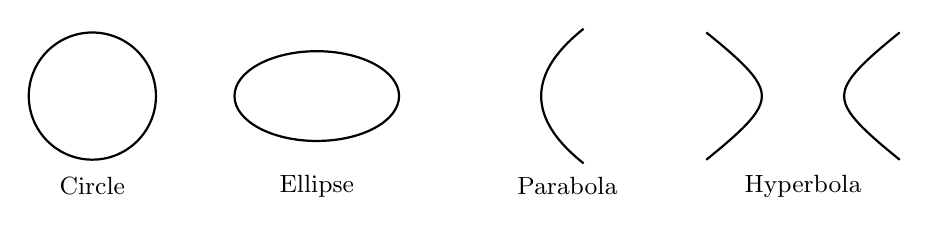
\begin{tikzpicture}[>=Stealth, scale=0.95]
  % Circle
  \draw[thick] (0,0) ellipse (0.85 and 0.85);
  \node at (0,-1.2) {\small Circle};
  % Ellipse
  \draw[thick] (3,0) ellipse (1.1 and 0.6);
  \node at (3,-1.2) {\small Ellipse};
  % Parabola
  \draw[thick,domain=-0.9:0.9,smooth,samples=30]
    plot ({6+\x*\x*0.7},\x);
  \node at (6.35,-1.2) {\small Parabola};
  % Hyperbola
  \draw[thick,domain=-0.75:0.75,smooth,samples=30]
    plot ({9.5+0.55*cosh(\x*2)},{sinh(\x*2)*0.4});
  \draw[thick,domain=-0.75:0.75,smooth,samples=30]
    plot ({9.5-0.55*cosh(\x*2)},{sinh(\x*2)*0.4});
  \node at (9.5,-1.2) {\small Hyperbola};
\end{tikzpicture}
\caption{The four main types of conic sections.}
\label{fig:731}
\end{figure}

Quadratic forms in $R^2$ arise naturally in the study of conics. An equation of the form
\begin{equation}
  ax^2+2bxy+cy^2+dx+ey+f=0 \tag{7}
\end{equation}
(with $a,b,c$ not all zero) represents a conic section. If $d=e=0$, Equation (7) becomes
\begin{equation}
  ax^2+2bxy+cy^2+f=0 \tag{8}
\end{equation}
a \textbf{central conic} (includes circles, ellipses, and hyperbolas, but not parabolas). If
further $b=0$:
\begin{equation}
  ax^2+cy^2+f=0 \tag{9}
\end{equation}
this is a \textbf{central conic in standard position}. The most important types are:

\begin{center}
\renewcommand{\arraystretch}{1.6}
\begin{tabular}{|l|c|l|}
\hline
\textbf{Type} & \textbf{Equation} & \textbf{Conditions}\\
\hline
Ellipse (major axis along $x$) & $\dfrac{x^2}{\alpha^2}+\dfrac{y^2}{\beta^2}=1$ & $\alpha\ge\beta>0$\\
\hline
Ellipse (major axis along $y$) & $\dfrac{x^2}{\alpha^2}+\dfrac{y^2}{\beta^2}=1$ & $\beta\ge\alpha>0$\\
\hline
Hyperbola (opens left/right) & $\dfrac{x^2}{\alpha^2}-\dfrac{y^2}{\beta^2}=1$ & $\alpha>0,\;\beta>0$\\
\hline
Hyperbola (opens up/down) & $\dfrac{y^2}{\beta^2}-\dfrac{x^2}{\alpha^2}=1$ & $\alpha>0,\;\beta>0$\\
\hline
\end{tabular}
\end{center}
\vspace{2mm}

Setting $k=-f$ and expressing (8) and (9) in matrix form:
\begin{equation}
  [x\;\;y]\begin{bmatrix}a&b\\b&c\end{bmatrix}\begin{bmatrix}x\\y\end{bmatrix}=k
  \quad\text{and}\quad
  [x\;\;y]\begin{bmatrix}a&0\\0&c\end{bmatrix}\begin{bmatrix}x\\y\end{bmatrix}=k \tag{10}
\end{equation}
A cross product term ($b\neq0$) signals that the graph is rotated out of standard position.
The three-dimensional analogs are:
\begin{equation}
  [x\;y\;z]\begin{bmatrix}a&d&e\\d&b&f\\e&f&c\end{bmatrix}\begin{bmatrix}x\\y\\z\end{bmatrix}=k
  \quad\text{and}\quad
  [x\;y\;z]\begin{bmatrix}a&0&0\\0&b&0\\0&0&c\end{bmatrix}\begin{bmatrix}x\\y\\z\end{bmatrix}=k \tag{11}
\end{equation}
The graphs of these in $R^3$ (when $a,b,c$ not all zero) are called \textbf{central quadrics};
the second is a \textbf{central quadric in standard position}.

\redheading{Identifying Conic Sections}

A central conic $ax^2+2bxy+cy^2=k$ is in standard position if $b=0$. When $b\neq0$, we can
identify the conic by writing the equation as
\begin{equation}
  \mathbf{x}^T A\mathbf{x}=k,\quad A=\begin{bmatrix}a&b\\b&c\end{bmatrix} \tag{13}
\end{equation}
and finding an orthogonal change of variable $\mathbf{x}=P\mathbf{x}'$ with $\det(P)=1$
(a rotation) that diagonalizes $A$. In the rotated $x'y'$-coordinate system, (13) becomes
\begin{equation}
  \mathbf{x}'^T D\mathbf{x}'=k,\quad\text{i.e.,}\quad \lambda_1x'^2+\lambda_2y'^2=k \tag{17}
\end{equation}
where $\lambda_1,\lambda_2$ are the eigenvalues of $A$. The first column of $P$ (a unit eigenvector
for $\lambda_1$) gives the direction of the positive $x'$-axis. A useful formula: when $b\neq0$, the
rotation angle $\theta$ satisfies
\begin{equation}
  \boxed{\cot 2\theta = \frac{a-c}{2b}} \tag{19}
\end{equation}

\subsection*{EXAMPLE 3 | Identifying a Conic by Eliminating the Cross Product Term}

\textbf{(a)} Identify the conic $5x^2-4xy+8y^2-36=0$ by rotating the $xy$-axes to standard
position.\\ \textbf{(b)} Find the angle $\theta$ of rotation.

\textbf{SOLUTION (a):} Write as $\mathbf{x}^T A\mathbf{x}=36$ with
\[
  A=\begin{bmatrix}5&-2\\-2&8\end{bmatrix}
\]
The characteristic polynomial of $A$ is
\[
  \begin{vmatrix}\lambda-5&2\\2&\lambda-8\end{vmatrix}=(\lambda-4)(\lambda-9)
\]
so the eigenvalues are $\lambda=4$ and $\lambda=9$. Orthonormal bases for the eigenspaces are:
\[
  \lambda=4:\;\begin{bmatrix}2/\sqrt{5}\\1/\sqrt{5}\end{bmatrix},\quad
  \lambda=9:\;\begin{bmatrix}-1/\sqrt{5}\\2/\sqrt{5}\end{bmatrix}
\]
Thus $A$ is orthogonally diagonalized by
\begin{equation}
  P=\begin{bmatrix}2/\sqrt{5}&-1/\sqrt{5}\\1/\sqrt{5}&2/\sqrt{5}\end{bmatrix} \tag{18}
\end{equation}
Since $\det(P)=1$, the substitution $\mathbf{x}=P\mathbf{x}'$ is a rotation. In the $x'y'$-system:
\[
  [x'\;\;y']\begin{bmatrix}4&0\\0&9\end{bmatrix}\begin{bmatrix}x'\\y'\end{bmatrix}=36
  \;\Rightarrow\; 4x'^2+9y'^2=36 \;\Rightarrow\; \frac{x'^2}{9}+\frac{y'^2}{4}=1
\]
This is an ellipse with major axis of length $2\alpha=6$ in the $x'$-direction and minor axis
of length $2\beta=4$ in the $y'$-direction.

\textbf{SOLUTION (b):} From (18), $\cos\theta=2/\sqrt{5}$ and $\sin\theta=1/\sqrt{5}$, so
\[
  \tan\theta = \frac{\sin\theta}{\cos\theta} = \frac{1}{2},\quad
  \theta = \tan^{-1}\tfrac{1}{2}\approx 26.6°
\]

\begin{figure}[ht]
\centering
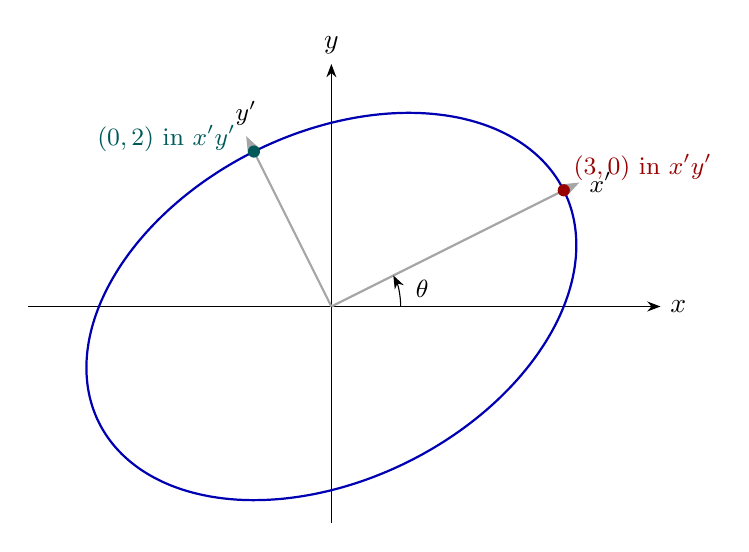
\begin{tikzpicture}[>=Stealth, scale=1.1]
  \draw[->] (-3.5,0)--(3.8,0) node[right]{$x$};
  \draw[->] (0,-2.5)--(0,2.8) node[above]{$y$};
  % Rotated axes (theta ~ 26.6 deg)
  \def\ct{0.8944}\def\st{0.4472}
  \draw[->,gray!70,thick] (0,0)--({3.2*\ct},{3.2*\st}) node[right,black]{\small$x'$};
  \draw[->,gray!70,thick] (0,0)--({-2.2*\st},{2.2*\ct}) node[above,black]{\small$y'$};
  % Ellipse in rotated frame: semi-axes a=3, b=2
  % Parametric: (3cos t * cos theta - 2 sin t * sin theta, 3 cos t * sin theta + 2 sin t * cos theta)
  \draw[thick,blue!70!black,domain=0:360,smooth,samples=100]
    plot ({3*cos(\x)*\ct - 2*sin(\x)*\st},{3*cos(\x)*\st + 2*sin(\x)*\ct});
  % Label eigenspace directions
  \fill[red!60!black] ({3*\ct},{3*\st}) circle (2pt) node[above right]{\small$(3,0)$ in $x'y'$};
  \fill[teal!70!black] ({-2*\st},{2*\ct}) circle (2pt);
  \node[teal!70!black] at ({-2*\st-0.1},{2*\ct+0.15}) [left]{\small$(0,2)$ in $x'y'$};
  % angle label
  \draw[->] (0.8,0) arc (0:26.6:0.8);
  \node at (1.05,0.2) {\small$\theta$};
\end{tikzpicture}
\caption{The ellipse $5x^2-4xy+8y^2=36$ in the original $xy$-frame, with the rotated
$x'y'$-axes along the principal axes.}
\label{fig:735}
\end{figure}

\redheading{Positive Definite Quadratic Forms}

We now consider Problem 2: conditions under which $\mathbf{x}^T A\mathbf{x}>0$ for all
$\mathbf{x}\neq\mathbf{0}$.

\begin{tcolorbox}[colback=teal!4, colframe=teal!65!black,
  title={\textbf{Definition 1}}, boxrule=0.5mm, arc=3mm]
A quadratic form $\mathbf{x}^T A\mathbf{x}$ (and the matrix $A$) is called:
\begin{itemize}
  \item \textbf{positive definite} if $\mathbf{x}^T A\mathbf{x}>0$ for all $\mathbf{x}\neq\mathbf{0}$
  \item \textbf{negative definite} if $\mathbf{x}^T A\mathbf{x}<0$ for all $\mathbf{x}\neq\mathbf{0}$
  \item \textbf{indefinite} if $\mathbf{x}^T A\mathbf{x}$ takes both positive and negative values
\end{itemize}
\end{tcolorbox}

\begin{tcolorbox}[colback=red!4, colframe=red!60!black,
  title={\textbf{Theorem 7.3.2}}, boxrule=0.5mm, arc=3mm]
If $A$ is a symmetric matrix, then:
\begin{enumerate}
  \item[(a)] $\mathbf{x}^T A\mathbf{x}$ is positive definite iff all eigenvalues of $A$ are positive.
  \item[(b)] $\mathbf{x}^T A\mathbf{x}$ is negative definite iff all eigenvalues of $A$ are negative.
  \item[(c)] $\mathbf{x}^T A\mathbf{x}$ is indefinite iff $A$ has at least one positive and at least
             one negative eigenvalue.
\end{enumerate}
\end{tcolorbox}

\textit{Proof.} By Theorem 7.3.1 there is an orthogonal change of variable $\mathbf{x}=P\mathbf{y}$ with
\begin{equation}
  \mathbf{x}^T A\mathbf{x} = \mathbf{y}^T D\mathbf{y}
  = \lambda_1y_1^2+\lambda_2y_2^2+\cdots+\lambda_ny_n^2 \tag{23}
\end{equation}
Since $P$ is invertible, $\mathbf{y}\neq\mathbf{0}\Leftrightarrow\mathbf{x}\neq\mathbf{0}$,
and the set of values of $\mathbf{x}^T A\mathbf{x}$ over all $\mathbf{x}$ equals the set of
values of $\mathbf{y}^T D\mathbf{y}$ over all $\mathbf{y}$.

\textbf{(a) and (b):} If all $\lambda_i>0$, then (23) is positive for every $\mathbf{y}\neq\mathbf{0}$,
so $\mathbf{x}^T A\mathbf{x}>0$. Conversely, if some $\lambda_i\le0$, taking $\mathbf{y}$ with
$y_i=1$ and all other $y_j=0$ gives $\mathbf{x}^T A\mathbf{x}=\lambda_i\le0$. Part (b) is
analogous.

\textbf{(c):} If $\lambda_1>0$ and $\lambda_2<0$, setting $y_1=1,y_2=\cdots=0$ gives
$\mathbf{x}^T A\mathbf{x}=\lambda_1>0$, and setting $y_2=1,y_1=y_3=\cdots=0$ gives
$\mathbf{x}^T A\mathbf{x}=\lambda_2<0$. Conversely, if both signs occur in (23), at least one
$\lambda_i$ must be positive and one negative. $\blacksquare$

\textit{Remark.} Two additional classifications:
\begin{itemize}
  \item $\mathbf{x}^T A\mathbf{x}$ is \textbf{positive semidefinite} if $\mathbf{x}^T A\mathbf{x}\ge0$
        for $\mathbf{x}\neq\mathbf{0}$ (all eigenvalues $\ge0$)
  \item $\mathbf{x}^T A\mathbf{x}$ is \textbf{negative semidefinite} if $\mathbf{x}^T A\mathbf{x}\le0$
        for $\mathbf{x}\neq\mathbf{0}$ (all eigenvalues $\le0$)
\end{itemize}

\subsection*{EXAMPLE 4 | Positive Definite Quadratic Forms}

Determine whether $\mathbf{x}^T A\mathbf{x}$ is positive definite for
$A=\begin{bmatrix}3&1&1\\1&0&2\\1&2&0\end{bmatrix}$.

\textbf{SOLUTION:} The entries are nonnegative, but the eigenvalues are $\lambda=1,4,-2$
(verify). Since $A$ has a negative eigenvalue, $\mathbf{x}^T A\mathbf{x}$ is indefinite.
Writing out the QF:
\[
  \mathbf{x}^T A\mathbf{x} = 3x_1^2+2x_1x_2+2x_1x_3+4x_2x_3
\]
Indeed, $\mathbf{x}^T A\mathbf{x}=4$ for $(x_1,x_2,x_3)=(0,1,1)$ and $\mathbf{x}^T A\mathbf{x}=-4$
for $(0,1,-1)$.

\redheading{Classifying Conic Sections Using Eigenvalues}

If $\mathbf{x}^T B\mathbf{x}=k$ with $k\neq0$, set $A=(1/k)B$ and rewrite as
\begin{equation}
  \mathbf{x}^T A\mathbf{x}=1 \tag{20}
\end{equation}
After rotating to eliminate cross product terms, (20) becomes
\begin{equation}
  \lambda_1x'^2+\lambda_2y'^2=1 \tag{21}
\end{equation}
where $\lambda_1,\lambda_2$ are eigenvalues of $A$:
\begin{itemize}
  \item Ellipse if $\lambda_1>0$ and $\lambda_2>0$
  \item No graph if $\lambda_1<0$ and $\lambda_2<0$
  \item Hyperbola if $\lambda_1,\lambda_2$ have opposite signs
\end{itemize}
For the ellipse case, (21) can be written
\begin{equation}
  \frac{x'^2}{(1/\sqrt{\lambda_1})^2}+\frac{y'^2}{(1/\sqrt{\lambda_2})^2}=1 \tag{22}
\end{equation}
so the axes have lengths $2/\sqrt{\lambda_1}$ and $2/\sqrt{\lambda_2}$.

\begin{tcolorbox}[colback=red!4, colframe=red!60!black,
  title={\textbf{Theorem 7.3.3}}, boxrule=0.5mm, arc=3mm]
If $A$ is a symmetric $2\times2$ matrix, then:
\begin{enumerate}
  \item[(a)] $\mathbf{x}^T A\mathbf{x}=1$ represents an ellipse if $A$ is positive definite.
  \item[(b)] $\mathbf{x}^T A\mathbf{x}=1$ has no graph if $A$ is negative definite.
  \item[(c)] $\mathbf{x}^T A\mathbf{x}=1$ represents a hyperbola if $A$ is indefinite.
\end{enumerate}
\end{tcolorbox}

\redheading{Identifying Positive Definite Matrices}

The \textbf{$k$th principal submatrix} of an $n\times n$ matrix $A$ is the $k\times k$ submatrix
formed by the first $k$ rows and columns of $A$. For a $4\times4$ matrix these are:

\[
  \begin{bmatrix}a_{11}\end{bmatrix},\quad
  \begin{bmatrix}a_{11}&a_{12}\\a_{21}&a_{22}\end{bmatrix},\quad
  \begin{bmatrix}a_{11}&a_{12}&a_{13}\\a_{21}&a_{22}&a_{23}\\a_{31}&a_{32}&a_{33}\end{bmatrix},\quad
  A
\]

\begin{tcolorbox}[colback=red!4, colframe=red!60!black,
  title={\textbf{Theorem 7.3.4}}, boxrule=0.5mm, arc=3mm]
If $A$ is a symmetric matrix, then:
\begin{enumerate}
  \item[(a)] $A$ is positive definite iff the determinant of every principal submatrix is positive.
  \item[(b)] $A$ is negative definite iff the determinants of the principal submatrices alternate
             in sign, beginning with a negative value.
  \item[(c)] $A$ is indefinite iff it is neither positive nor negative definite and at least one
             principal submatrix has a positive determinant and at least one has a negative
             determinant.
\end{enumerate}
\end{tcolorbox}

\subsection*{EXAMPLE 5 | Working with Principal Submatrices}

The matrix
\[
  A=\begin{bmatrix}2&-1&-3\\-1&2&4\\-3&4&9\end{bmatrix}
\]
is positive definite since its principal submatrix determinants
\[
  |2|=2,\quad
  \begin{vmatrix}2&-1\\-1&2\end{vmatrix}=3,\quad
  \begin{vmatrix}2&-1&-3\\-1&2&4\\-3&4&9\end{vmatrix}=1
\]
are all positive. Thus all eigenvalues of $A$ are positive and $\mathbf{x}^T A\mathbf{x}>0$
for all $\mathbf{x}\neq\mathbf{0}$.

\vspace{3mm}
\noindent\rule{\linewidth}{0.5pt}

\section*{Exercise Set 7.3}

\noindent\textit{In Exercises 1--2, express the quadratic form in the matrix notation
$\mathbf{x}^T A\mathbf{x}$, where $A$ is symmetric.}

\begin{enumerate}

\item \textbf{a.}\ $3x_1^2+7x_2^2$
\hspace{20pt}
\textbf{b.}\ $4x_1^2-9x_2^2-6x_1x_2$

\quad\textbf{c.}\ $9x_1^2-x_2^2+4x_3^2+6x_1x_2-8x_1x_3+x_2x_3$

\noindent\textit{In Exercises 3--4, find a formula for the quadratic form that does not use
matrices.}

\item[3.] $[x\;\;y]\begin{bmatrix}2&-3\\-3&5\end{bmatrix}\begin{bmatrix}x\\y\end{bmatrix}$

\noindent\textit{In Exercises 5--8, find an orthogonal change of variables that eliminates the
cross product terms in $Q$, and express $Q$ in terms of the new variables.}

\item[5.] $Q = 2x_1^2+2x_2^2-2x_1x_2$

\item[7.] $Q = 3x_1^2+4x_2^2+5x_3^2+4x_1x_2-4x_2x_3$

\noindent\textit{In Exercises 9--10, express the quadratic equation in the matrix form
$\mathbf{x}^T A\mathbf{x}+K\mathbf{x}+f=0$, where $\mathbf{x}^T A\mathbf{x}$ is the associated
quadratic form and $K$ is an appropriate matrix.}

\item[9.] \textbf{a.}\ $2x^2+xy+x-6y+2=0$
\hspace{20pt}
\textbf{b.}\ $y^2+7x-8y-5=0$

\noindent\textit{In Exercises 11--12, identify the conic section represented by the equation.}

\item[11.] \textbf{a.}\ $2x^2+5y^2=20$
\hspace{20pt}
\textbf{b.}\ $x^2-y^2-8=0$
\hspace{20pt}
\textbf{c.}\ $7y^2-2x=0$

\noindent\textit{In Exercises 13--16, identify the conic section by rotating axes to place it in
standard position. Find the equation in the rotated coordinates and the angle of rotation.}

\item[13.] $2x^2-4xy-y^2+8=0$

\item[16.] $x^2+xy+y^2=\tfrac{1}{2}$

\noindent\textit{In Exercises 17--18, determine by inspection whether the matrix is positive
definite, negative definite, indefinite, positive semidefinite, or negative semidefinite.}

\item[17.]
\textbf{a.}\ $\begin{bmatrix}1&0\\0&2\end{bmatrix}$
\hspace{15pt}
\textbf{b.}\ $\begin{bmatrix}-1&0\\0&-2\end{bmatrix}$
\hspace{15pt}
\textbf{c.}\ $\begin{bmatrix}-1&0\\0&2\end{bmatrix}$
\hspace{15pt}
\textbf{d.}\ $\begin{bmatrix}1&0\\0&0\end{bmatrix}$
\hspace{15pt}
\textbf{e.}\ $\begin{bmatrix}0&0\\0&-2\end{bmatrix}$

\noindent\textit{In Exercises 19--24, classify the quadratic form as positive definite, negative
definite, indefinite, positive semidefinite, or negative semidefinite.}

\item[19.] $x_1^2+x_2^2$

\item[22.] $-(x_1-x_2)^2$

\noindent\textit{In Exercises 25--26, show that $A$ is positive definite first by using
Theorem 7.3.2 and then by using Theorem 7.3.4.}

\item[25.] \textbf{a.}\ $A=\begin{bmatrix}5&-2\\-2&5\end{bmatrix}$
\hspace{20pt}
\textbf{b.}\ $A=\begin{bmatrix}2&-1&0\\-1&2&0\\0&0&5\end{bmatrix}$

\item[26.] \textbf{a.}\ $A=\begin{bmatrix}2&1\\1&2\end{bmatrix}$
\hspace{20pt}
\textbf{b.}\ $A=\begin{bmatrix}3&-1&0\\-1&2&0\\0&0&5\end{bmatrix}$

\noindent\textit{In Exercises 27--28, use Theorem 7.3.4 to classify the matrix as positive
definite, negative definite, or indefinite.}

\item[27.] \textbf{a.}\ $A=\begin{bmatrix}3&1&2\\1&-1&3\\2&3&2\end{bmatrix}$
\hspace{20pt}
\textbf{b.}\ $A=\begin{bmatrix}-3&2&0\\2&-3&0\\0&0&-5\end{bmatrix}$

\noindent\textit{In Exercises 29--30, find all values of $k$ for which the quadratic form is
positive definite.}

\item[29.] $5x_1^2+x_2^2+kx_3^2+4x_1x_2-2x_1x_3-2x_2x_3$

\noindent\textit{\textbf{Working with Proofs}}

\item[31.] Let $\mathbf{x}^T A\mathbf{x}$ be a quadratic form in $x_1,\ldots,x_n$, and define
$T\colon R^n\to R$ by $T(\mathbf{x})=\mathbf{x}^T A\mathbf{x}$.

\textbf{a.}\ Show that $T(\mathbf{x}+\mathbf{y})=T(\mathbf{x})+2\mathbf{x}^T A\mathbf{y}+T(\mathbf{y})$.

\textbf{b.}\ Show that $T(c\mathbf{x})=c^2T(\mathbf{x})$.

\item[33.] In statistics, the \emph{sample mean} and \emph{sample variance} of $\mathbf{x}=(x_1,\ldots,x_n)$ are
\[
  \bar{x}=\tfrac{1}{n}(x_1+\cdots+x_n),\quad
  s_x^2=\tfrac{1}{n-1}\bigl[(x_1-\bar{x})^2+\cdots+(x_n-\bar{x})^2\bigr]
\]
\textbf{a.}\ Express $s_x^2$ in matrix notation $\mathbf{x}^T A\mathbf{x}$ where $A$ is symmetric.

\textbf{b.}\ Is $s_x^2$ a positive definite quadratic form? Explain.

\item[36.] Prove: if $b\neq0$, the cross product term in $ax^2+2bxy+cy^2=k$ can be eliminated by
rotating through an angle $\theta$ satisfying $\cot 2\theta=\dfrac{a-c}{2b}$.

\end{enumerate}

\end{document}
